\section{细分曲面}\label{sec:细分曲面}
\begin{remark}
    本节含有高级内容,第一次阅读时可以跳过。
\end{remark}

本章我们要定义的最后一个形状表示
实现了\keyindex{细分曲面}{subdivision surface}{surface曲面},
该表示尤其适合描述复杂光滑形状。
特定网格的细分曲面定义为将网格面反复细分为更小面
然后用旧顶点位置的加权组合求新顶点位置。

对于适当选择的细分规则,当细分步数趋于无穷时,
该过程会收敛到给出一个光滑的\keyindex{极限曲面}{limit surface}{surface曲面}。
实践中,只需少量级别的细分通常就足以得到极限曲面的良好近似。
\reffig{3.24}展示了一个细分的简单例子,
其中四面体被细分了零次、一次、两次和六次。
\begin{figure}[htbp]
    \centering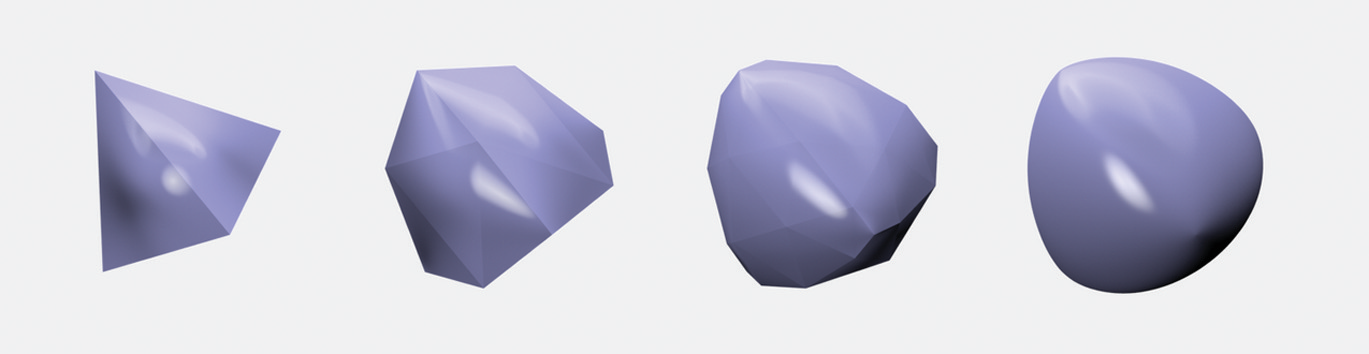
\includegraphics[width=\linewidth]{chap03/tetsubdiv.png}
    \caption{四面体的细分。从左到右使用了零步、一步、两步和六步细分
        (在零级时,顶点只是移动到极限曲面上)。
        随着细分得越来越多,网格逼近极限曲面,即原始网格描述的光滑曲面。
        随着执行更多级别的细分,注意高光如何变得更加准确、轮廓边缘如何变得更加平滑。}
    \label{fig:3.24}
\end{figure}

\reffig{3.25}展示了对Killeroo\sidenote{译者注:猜测此名字与一澳大利亚漫画中的袋鼠角色名有关。}模型应用细分的效果;
上面是原始控制网格,下面是控制网格表示的细分曲面。
\begin{figure}[htbp]
    \centering
    \subfloat[控制网格]{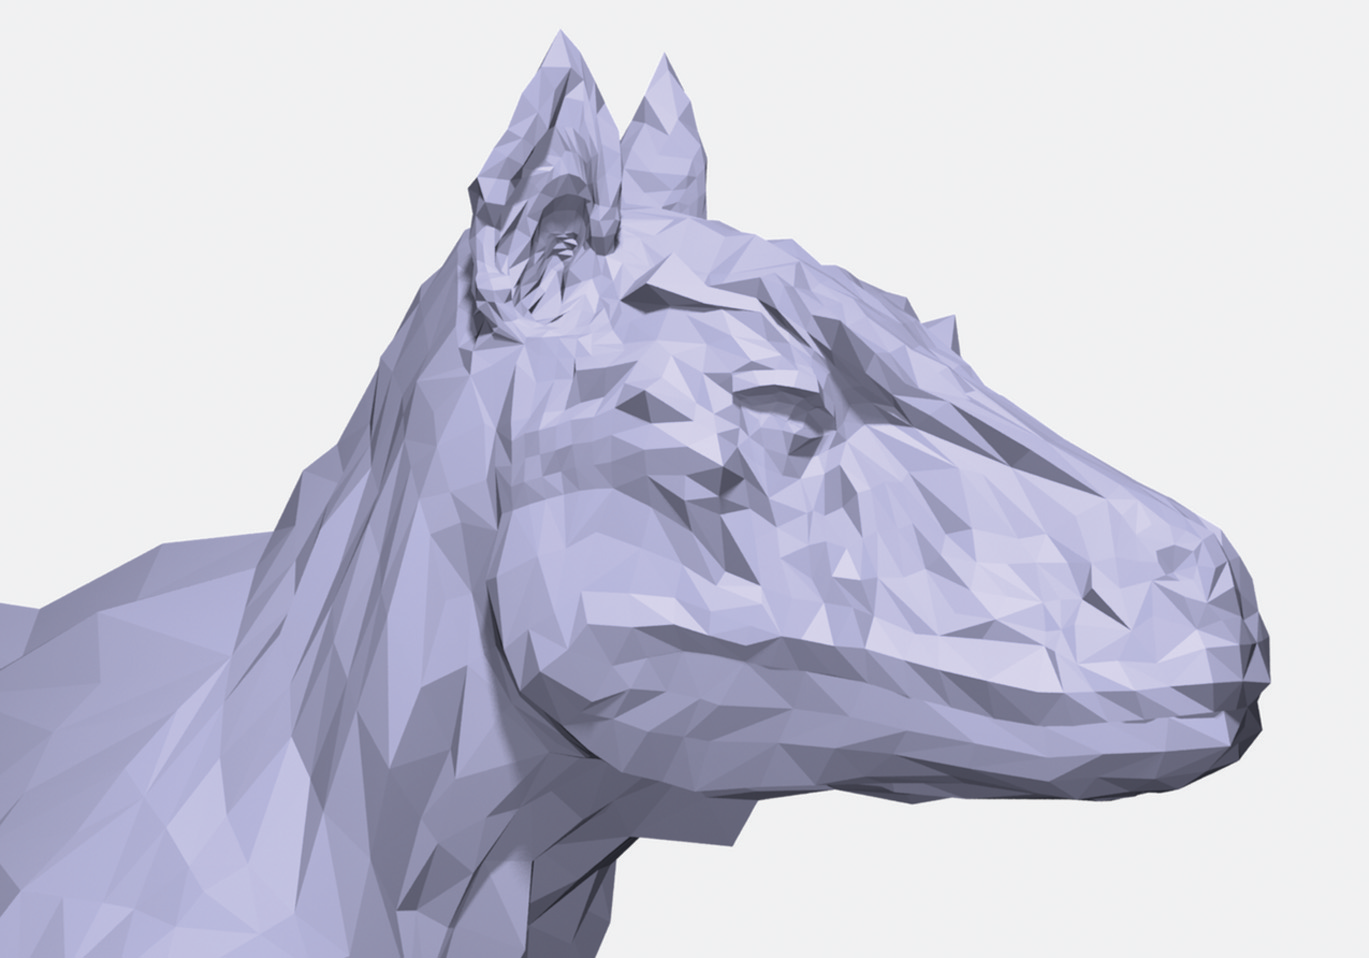
\includegraphics[width=\linewidth]{chap03/killeroo-control.png}\label{fig:3.25.1}}\\
    \subfloat[细分网格]{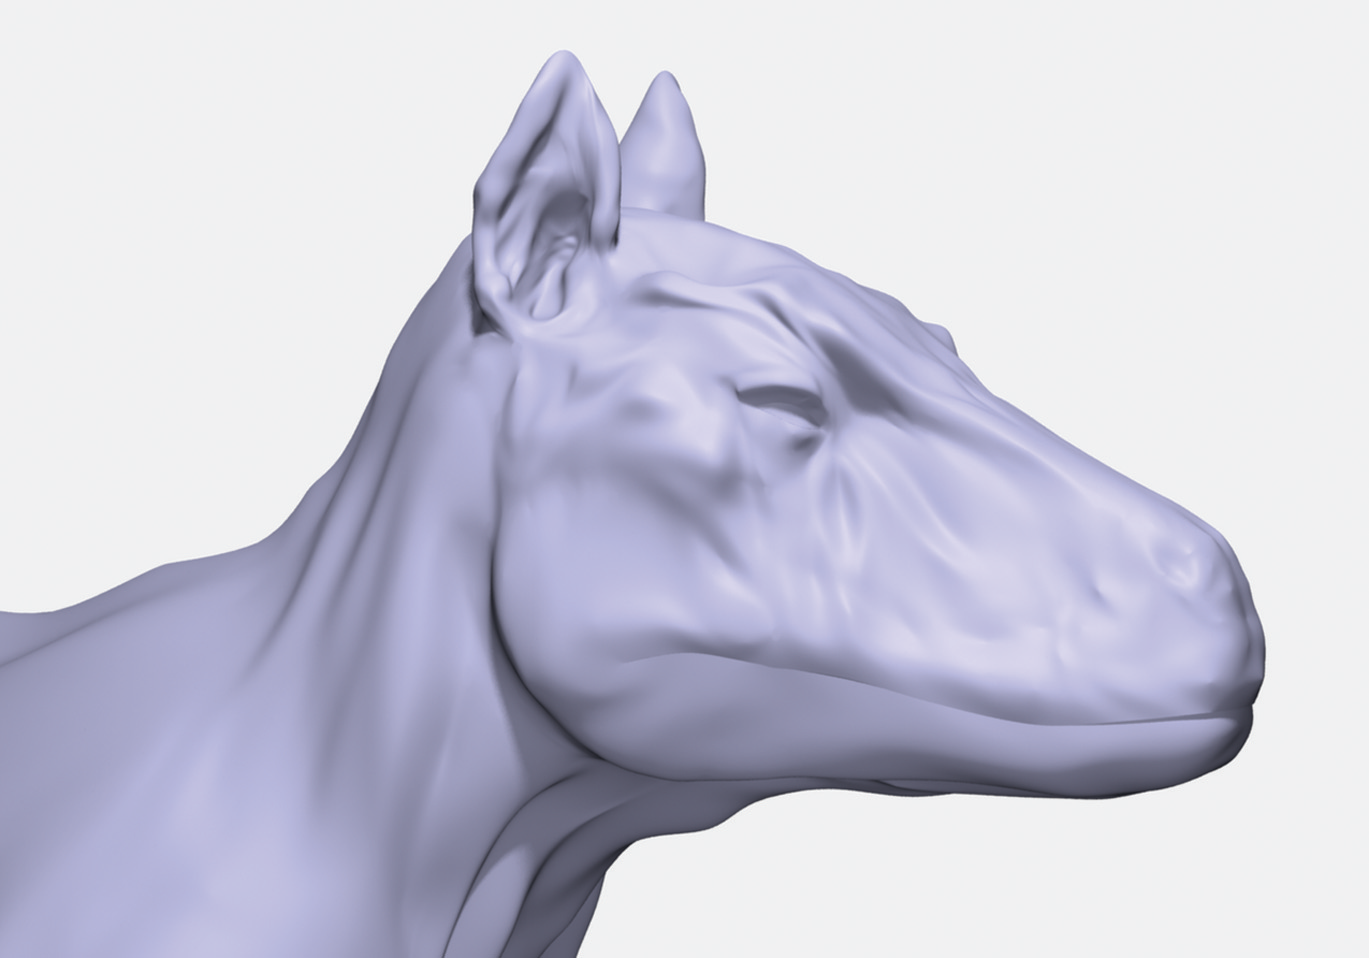
\includegraphics[width=\linewidth]{chap03/killeroo-subdivided.png}\label{fig:3.25.2}}
    \caption{对Killeroo模型应用细分。(1)控制网格描述了(2)结果细分曲面。
        细分非常适合建模这样的形状,因为它能通过细化控制网格轻松添加局部细节,
        对最终曲面没有拓扑结构限制。(模型由headus/Rezard提供。)}
    \label{fig:3.25}
\end{figure}


因为在曲面的多边形和基于样条的表示方面有一些重要优势,
细分曲面近年来得到广泛运用,尽管它在20世纪70年代就被发明了。
细分的优势包括:
\begin{itemize}
    \item 细分曲面是平滑的,而多边形网格与之相反,无论建模得多细致,靠近观察会有小面。
    \item 建模系统中现有的多数基本结构可以重定向到细分。
          建模多边形网格的经典技术工具箱可以应用到建模细分控制网格上。
    \item 细分曲面非常适合描述有复杂拓扑结构的物体,
          因为它们以任意(\keyindex{流形}{manifold}{})拓扑结构的控制网格为起点。
          参数化曲面模型一般不能很好地处理复杂拓扑结构。
    \item 细分方法常常是基于样条的曲面表示的推广,
          所以样条曲面常常可以由通用细分曲面渲染器运行。
    \item 通过简单地对控制网格的适当部分添加面,它能轻松对细分曲面局部区域添加细节。
          用样条表示则要困难得多。
\end{itemize}
\begin{figure}[htbp]
    \centering%LaTeX with PSTricks extensions
%%Creator: Inkscape 1.0.1 (3bc2e813f5, 2020-09-07)
%%Please note this file requires PSTricks extensions
\psset{xunit=.5pt,yunit=.5pt,runit=.5pt}
\begin{pspicture}(487.94000244,169.97000122)
{
\newrgbcolor{curcolor}{0.7019608 0.7019608 0.7019608}
\pscustom[linestyle=none,fillstyle=solid,fillcolor=curcolor]
{
\newpath
\moveto(96.28,168.97000122)
\lineto(143.98,86.34000122)
\lineto(191.69,3.72000122)
\lineto(96.28,3.72000122)
\lineto(0.87,3.72000122)
\lineto(48.57,86.34000122)
\closepath
}
}
{
\newrgbcolor{curcolor}{0 0 0}
\pscustom[linewidth=1,linecolor=curcolor]
{
\newpath
\moveto(96.28,168.97000122)
\lineto(143.98,86.34000122)
\lineto(191.69,3.72000122)
\lineto(96.28,3.72000122)
\lineto(0.87,3.72000122)
\lineto(48.57,86.34000122)
\closepath
}
}
{
\newrgbcolor{curcolor}{0.7019608 0.7019608 0.7019608}
\pscustom[linestyle=none,fillstyle=solid,fillcolor=curcolor]
{
\newpath
\moveto(96.28,4.73000122)
\lineto(72.9,45.22000122)
\lineto(49.52,85.71000122)
\lineto(96.28,85.71000122)
\lineto(143.03,85.71000122)
\lineto(119.65,45.22000122)
\closepath
}
}
{
\newrgbcolor{curcolor}{0 0 0}
\pscustom[linewidth=0.5,linecolor=curcolor]
{
\newpath
\moveto(96.28,4.73000122)
\lineto(72.9,45.22000122)
\lineto(49.52,85.71000122)
\lineto(96.28,85.71000122)
\lineto(143.03,85.71000122)
\lineto(119.65,45.22000122)
\closepath
}
}
{
\newrgbcolor{curcolor}{0.7019608 0.7019608 0.7019608}
\pscustom[linestyle=none,fillstyle=solid,fillcolor=curcolor]
{
\newpath
\moveto(391.67,168.97000122)
\lineto(439.37,86.34000122)
\lineto(487.08,3.72000122)
\lineto(391.67,3.72000122)
\lineto(296.26,3.72000122)
\lineto(343.96,86.34000122)
\closepath
}
}
{
\newrgbcolor{curcolor}{0 0 0}
\pscustom[linewidth=1,linecolor=curcolor]
{
\newpath
\moveto(391.67,168.97000122)
\lineto(439.37,86.34000122)
\lineto(487.08,3.72000122)
\lineto(391.67,3.72000122)
\lineto(296.26,3.72000122)
\lineto(343.96,86.34000122)
\closepath
}
}
{
\newrgbcolor{curcolor}{0.7019608 0.7019608 0.7019608}
\pscustom[linestyle=none,fillstyle=solid,fillcolor=curcolor]
{
\newpath
\moveto(391.67,4.73000122)
\lineto(368.29,45.22000122)
\lineto(344.92,85.71000122)
\lineto(391.67,85.71000122)
\lineto(438.42,85.71000122)
\lineto(415.04,45.22000122)
\closepath
}
}
{
\newrgbcolor{curcolor}{0 0 0}
\pscustom[linewidth=0.5,linecolor=curcolor]
{
\newpath
\moveto(391.67,4.73000122)
\lineto(368.29,45.22000122)
\lineto(344.92,85.71000122)
\lineto(391.67,85.71000122)
\lineto(438.42,85.71000122)
\lineto(415.04,45.22000122)
\closepath
}
}
{
\newrgbcolor{curcolor}{0.7019608 0.7019608 0.7019608}
\pscustom[linestyle=none,fillstyle=solid,fillcolor=curcolor]
{
\newpath
\moveto(391.89,86.41000122)
\lineto(380.43,106.25000122)
\lineto(368.98,126.09000122)
\lineto(391.89,126.09000122)
\lineto(414.8,126.09000122)
\lineto(403.34,106.25000122)
\closepath
}
}
{
\newrgbcolor{curcolor}{0 0 0}
\pscustom[linewidth=0.5,linecolor=curcolor,linestyle=dashed,dash=2]
{
\newpath
\moveto(391.89,86.41000122)
\lineto(380.43,106.25000122)
\lineto(368.98,126.09000122)
\lineto(391.89,126.09000122)
\lineto(414.8,126.09000122)
\lineto(403.34,106.25000122)
\closepath
}
}
{
\newrgbcolor{curcolor}{0.7019608 0.7019608 0.7019608}
\pscustom[linestyle=none,fillstyle=solid,fillcolor=curcolor]
{
\newpath
\moveto(344.09,4.78000122)
\lineto(332.64,24.62000122)
\lineto(321.19,44.46000122)
\lineto(344.09,44.46000122)
\lineto(367,44.46000122)
\lineto(355.55,24.62000122)
\closepath
}
}
{
\newrgbcolor{curcolor}{0 0 0}
\pscustom[linewidth=0.5,linecolor=curcolor,linestyle=dashed,dash=2]
{
\newpath
\moveto(344.09,4.78000122)
\lineto(332.64,24.62000122)
\lineto(321.19,44.46000122)
\lineto(344.09,44.46000122)
\lineto(367,44.46000122)
\lineto(355.55,24.62000122)
\closepath
}
}
{
\newrgbcolor{curcolor}{0.7019608 0.7019608 0.7019608}
\pscustom[linestyle=none,fillstyle=solid,fillcolor=curcolor]
{
\newpath
\moveto(439.39,5.37000122)
\lineto(427.94,25.21000122)
\lineto(416.48,45.05000122)
\lineto(439.39,45.05000122)
\lineto(462.3,45.05000122)
\lineto(450.84,25.21000122)
\closepath
}
}
{
\newrgbcolor{curcolor}{0 0 0}
\pscustom[linewidth=0.5,linecolor=curcolor,linestyle=dashed,dash=2]
{
\newpath
\moveto(439.39,5.37000122)
\lineto(427.94,25.21000122)
\lineto(416.48,45.05000122)
\lineto(439.39,45.05000122)
\lineto(462.3,45.05000122)
\lineto(450.84,25.21000122)
\closepath
}
}
{
\newrgbcolor{curcolor}{0.7019608 0.7019608 0.7019608}
\pscustom[linestyle=none,fillstyle=solid,fillcolor=curcolor]
{
\newpath
\moveto(392.26,85.27000122)
\lineto(403.71,65.43000122)
\lineto(415.16,45.59000122)
\lineto(392.26,45.59000122)
\lineto(369.35,45.59000122)
\lineto(380.8,65.43000122)
\closepath
}
}
{
\newrgbcolor{curcolor}{0 0 0}
\pscustom[linewidth=0.5,linecolor=curcolor,linestyle=dashed,dash=2]
{
\newpath
\moveto(392.26,85.27000122)
\lineto(403.71,65.43000122)
\lineto(415.16,45.59000122)
\lineto(392.26,45.59000122)
\lineto(369.35,45.59000122)
\lineto(380.8,65.43000122)
\closepath
}
}
{
\newrgbcolor{curcolor}{0 0 0}
\pscustom[linestyle=none,fillstyle=solid,fillcolor=curcolor]
{
\newpath
\moveto(419.14999509,126.22999954)
\curveto(419.14999509,129.37511236)(415.34769602,130.94962069)(413.124035,128.72595966)
\curveto(410.90037397,126.50229864)(412.4748823,122.69999957)(415.61999512,122.69999957)
\curveto(418.76510794,122.69999957)(420.33961626,126.50229864)(418.11595524,128.72595966)
\curveto(415.89229421,130.94962069)(412.08999515,129.37511236)(412.08999515,126.22999954)
\curveto(412.08999515,123.08488672)(415.89229421,121.5103784)(418.11595524,123.73403942)
\curveto(420.33961626,125.95770045)(418.76510794,129.75999951)(415.61999512,129.75999951)
\curveto(412.4748823,129.75999951)(410.90037397,125.95770045)(413.124035,123.73403942)
\curveto(415.34769602,121.5103784)(419.14999509,123.08488672)(419.14999509,126.22999954)
\closepath
}
}
{
\newrgbcolor{curcolor}{0 0 0}
\pscustom[linewidth=1,linecolor=curcolor]
{
\newpath
\moveto(419.14999509,126.22999954)
\curveto(419.14999509,129.37511236)(415.34769602,130.94962069)(413.124035,128.72595966)
\curveto(410.90037397,126.50229864)(412.4748823,122.69999957)(415.61999512,122.69999957)
\curveto(418.76510794,122.69999957)(420.33961626,126.50229864)(418.11595524,128.72595966)
\curveto(415.89229421,130.94962069)(412.08999515,129.37511236)(412.08999515,126.22999954)
\curveto(412.08999515,123.08488672)(415.89229421,121.5103784)(418.11595524,123.73403942)
\curveto(420.33961626,125.95770045)(418.76510794,129.75999951)(415.61999512,129.75999951)
\curveto(412.4748823,129.75999951)(410.90037397,125.95770045)(413.124035,123.73403942)
\curveto(415.34769602,121.5103784)(419.14999509,123.08488672)(419.14999509,126.22999954)
\closepath
}
}
{
\newrgbcolor{curcolor}{0 0 0}
\pscustom[linestyle=none,fillstyle=solid,fillcolor=curcolor]
{
\newpath
\moveto(395.51001096,85.79000092)
\curveto(395.51001096,88.93511374)(391.70771189,90.50962206)(389.48405087,88.28596104)
\curveto(387.26038984,86.06230001)(388.83489817,82.26000094)(391.98001099,82.26000094)
\curveto(395.12512381,82.26000094)(396.69963213,86.06230001)(394.47597111,88.28596104)
\curveto(392.25231008,90.50962206)(388.45001101,88.93511374)(388.45001101,85.79000092)
\curveto(388.45001101,82.6448881)(392.25231008,81.07037977)(394.47597111,83.2940408)
\curveto(396.69963213,85.51770182)(395.12512381,89.32000089)(391.98001099,89.32000089)
\curveto(388.83489817,89.32000089)(387.26038984,85.51770182)(389.48405087,83.2940408)
\curveto(391.70771189,81.07037977)(395.51001096,82.6448881)(395.51001096,85.79000092)
\closepath
}
}
{
\newrgbcolor{curcolor}{0 0 0}
\pscustom[linewidth=1,linecolor=curcolor]
{
\newpath
\moveto(395.51001096,85.79000092)
\curveto(395.51001096,88.93511374)(391.70771189,90.50962206)(389.48405087,88.28596104)
\curveto(387.26038984,86.06230001)(388.83489817,82.26000094)(391.98001099,82.26000094)
\curveto(395.12512381,82.26000094)(396.69963213,86.06230001)(394.47597111,88.28596104)
\curveto(392.25231008,90.50962206)(388.45001101,88.93511374)(388.45001101,85.79000092)
\curveto(388.45001101,82.6448881)(392.25231008,81.07037977)(394.47597111,83.2940408)
\curveto(396.69963213,85.51770182)(395.12512381,89.32000089)(391.98001099,89.32000089)
\curveto(388.83489817,89.32000089)(387.26038984,85.51770182)(389.48405087,83.2940408)
\curveto(391.70771189,81.07037977)(395.51001096,82.6448881)(395.51001096,85.79000092)
\closepath
}
}
{
\newrgbcolor{curcolor}{0 0 0}
\pscustom[linestyle=none,fillstyle=solid,fillcolor=curcolor]
{
\newpath
\moveto(370.98999143,127.18000031)
\curveto(370.98999143,130.32511313)(367.18769236,131.89962145)(364.96403134,129.67596042)
\curveto(362.74037031,127.4522994)(364.31487864,123.65000033)(367.45999146,123.65000033)
\curveto(370.60510428,123.65000033)(372.1796126,127.4522994)(369.95595157,129.67596042)
\curveto(367.73229055,131.89962145)(363.92999148,130.32511313)(363.92999148,127.18000031)
\curveto(363.92999148,124.03488749)(367.73229055,122.46037916)(369.95595157,124.68404019)
\curveto(372.1796126,126.90770121)(370.60510428,130.71000028)(367.45999146,130.71000028)
\curveto(364.31487864,130.71000028)(362.74037031,126.90770121)(364.96403134,124.68404019)
\curveto(367.18769236,122.46037916)(370.98999143,124.03488749)(370.98999143,127.18000031)
\closepath
}
}
{
\newrgbcolor{curcolor}{0 0 0}
\pscustom[linewidth=1,linecolor=curcolor]
{
\newpath
\moveto(370.98999143,127.18000031)
\curveto(370.98999143,130.32511313)(367.18769236,131.89962145)(364.96403134,129.67596042)
\curveto(362.74037031,127.4522994)(364.31487864,123.65000033)(367.45999146,123.65000033)
\curveto(370.60510428,123.65000033)(372.1796126,127.4522994)(369.95595157,129.67596042)
\curveto(367.73229055,131.89962145)(363.92999148,130.32511313)(363.92999148,127.18000031)
\curveto(363.92999148,124.03488749)(367.73229055,122.46037916)(369.95595157,124.68404019)
\curveto(372.1796126,126.90770121)(370.60510428,130.71000028)(367.45999146,130.71000028)
\curveto(364.31487864,130.71000028)(362.74037031,126.90770121)(364.96403134,124.68404019)
\curveto(367.18769236,122.46037916)(370.98999143,124.03488749)(370.98999143,127.18000031)
\closepath
}
}
{
\newrgbcolor{curcolor}{0 0 0}
\pscustom[linestyle=none,fillstyle=solid,fillcolor=curcolor]
{
\newpath
\moveto(418.45999265,46.02999878)
\curveto(418.45999265,49.1751116)(414.65769358,50.74961993)(412.43403256,48.5259589)
\curveto(410.21037153,46.30229787)(411.78487986,42.49999881)(414.92999268,42.49999881)
\curveto(418.0751055,42.49999881)(419.64961382,46.30229787)(417.4259528,48.5259589)
\curveto(415.20229177,50.74961993)(411.3999927,49.1751116)(411.3999927,46.02999878)
\curveto(411.3999927,42.88488596)(415.20229177,41.31037763)(417.4259528,43.53403866)
\curveto(419.64961382,45.75769969)(418.0751055,49.55999875)(414.92999268,49.55999875)
\curveto(411.78487986,49.55999875)(410.21037153,45.75769969)(412.43403256,43.53403866)
\curveto(414.65769358,41.31037763)(418.45999265,42.88488596)(418.45999265,46.02999878)
\closepath
}
}
{
\newrgbcolor{curcolor}{0 0 0}
\pscustom[linewidth=1,linecolor=curcolor]
{
\newpath
\moveto(418.45999265,46.02999878)
\curveto(418.45999265,49.1751116)(414.65769358,50.74961993)(412.43403256,48.5259589)
\curveto(410.21037153,46.30229787)(411.78487986,42.49999881)(414.92999268,42.49999881)
\curveto(418.0751055,42.49999881)(419.64961382,46.30229787)(417.4259528,48.5259589)
\curveto(415.20229177,50.74961993)(411.3999927,49.1751116)(411.3999927,46.02999878)
\curveto(411.3999927,42.88488596)(415.20229177,41.31037763)(417.4259528,43.53403866)
\curveto(419.64961382,45.75769969)(418.0751055,49.55999875)(414.92999268,49.55999875)
\curveto(411.78487986,49.55999875)(410.21037153,45.75769969)(412.43403256,43.53403866)
\curveto(414.65769358,41.31037763)(418.45999265,42.88488596)(418.45999265,46.02999878)
\closepath
}
}
{
\newrgbcolor{curcolor}{0 0 0}
\pscustom[linestyle=none,fillstyle=solid,fillcolor=curcolor]
{
\newpath
\moveto(371.64999509,45.45000458)
\curveto(371.64999509,48.5951174)(367.84769602,50.16962572)(365.624035,47.9459647)
\curveto(363.40037397,45.72230367)(364.9748823,41.92000461)(368.11999512,41.92000461)
\curveto(371.26510794,41.92000461)(372.83961626,45.72230367)(370.61595524,47.9459647)
\curveto(368.39229421,50.16962572)(364.58999515,48.5951174)(364.58999515,45.45000458)
\curveto(364.58999515,42.30489176)(368.39229421,40.73038343)(370.61595524,42.95404446)
\curveto(372.83961626,45.17770548)(371.26510794,48.98000455)(368.11999512,48.98000455)
\curveto(364.9748823,48.98000455)(363.40037397,45.17770548)(365.624035,42.95404446)
\curveto(367.84769602,40.73038343)(371.64999509,42.30489176)(371.64999509,45.45000458)
\closepath
}
}
{
\newrgbcolor{curcolor}{0 0 0}
\pscustom[linewidth=1,linecolor=curcolor]
{
\newpath
\moveto(371.64999509,45.45000458)
\curveto(371.64999509,48.5951174)(367.84769602,50.16962572)(365.624035,47.9459647)
\curveto(363.40037397,45.72230367)(364.9748823,41.92000461)(368.11999512,41.92000461)
\curveto(371.26510794,41.92000461)(372.83961626,45.72230367)(370.61595524,47.9459647)
\curveto(368.39229421,50.16962572)(364.58999515,48.5951174)(364.58999515,45.45000458)
\curveto(364.58999515,42.30489176)(368.39229421,40.73038343)(370.61595524,42.95404446)
\curveto(372.83961626,45.17770548)(371.26510794,48.98000455)(368.11999512,48.98000455)
\curveto(364.9748823,48.98000455)(363.40037397,45.17770548)(365.624035,42.95404446)
\curveto(367.84769602,40.73038343)(371.64999509,42.30489176)(371.64999509,45.45000458)
\closepath
}
}
{
\newrgbcolor{curcolor}{0 0 0}
\pscustom[linestyle=none,fillstyle=solid,fillcolor=curcolor]
{
\newpath
\moveto(466.45999265,45.13999939)
\curveto(466.45999265,48.28511221)(462.65769358,49.85962054)(460.43403256,47.63595951)
\curveto(458.21037153,45.41229848)(459.78487986,41.60999942)(462.92999268,41.60999942)
\curveto(466.0751055,41.60999942)(467.64961382,45.41229848)(465.4259528,47.63595951)
\curveto(463.20229177,49.85962054)(459.3999927,48.28511221)(459.3999927,45.13999939)
\curveto(459.3999927,41.99488657)(463.20229177,40.42037824)(465.4259528,42.64403927)
\curveto(467.64961382,44.8677003)(466.0751055,48.66999936)(462.92999268,48.66999936)
\curveto(459.78487986,48.66999936)(458.21037153,44.8677003)(460.43403256,42.64403927)
\curveto(462.65769358,40.42037824)(466.45999265,41.99488657)(466.45999265,45.13999939)
\closepath
}
}
{
\newrgbcolor{curcolor}{0 0 0}
\pscustom[linewidth=1,linecolor=curcolor]
{
\newpath
\moveto(466.45999265,45.13999939)
\curveto(466.45999265,48.28511221)(462.65769358,49.85962054)(460.43403256,47.63595951)
\curveto(458.21037153,45.41229848)(459.78487986,41.60999942)(462.92999268,41.60999942)
\curveto(466.0751055,41.60999942)(467.64961382,45.41229848)(465.4259528,47.63595951)
\curveto(463.20229177,49.85962054)(459.3999927,48.28511221)(459.3999927,45.13999939)
\curveto(459.3999927,41.99488657)(463.20229177,40.42037824)(465.4259528,42.64403927)
\curveto(467.64961382,44.8677003)(466.0751055,48.66999936)(462.92999268,48.66999936)
\curveto(459.78487986,48.66999936)(458.21037153,44.8677003)(460.43403256,42.64403927)
\curveto(462.65769358,40.42037824)(466.45999265,41.99488657)(466.45999265,45.13999939)
\closepath
}
}
{
\newrgbcolor{curcolor}{0 0 0}
\pscustom[linestyle=none,fillstyle=solid,fillcolor=curcolor]
{
\newpath
\moveto(323.7000134,45.41999817)
\curveto(323.7000134,48.56511099)(319.89771433,50.13961932)(317.67405331,47.91595829)
\curveto(315.45039228,45.69229726)(317.02490061,41.8899982)(320.17001343,41.8899982)
\curveto(323.31512625,41.8899982)(324.88963457,45.69229726)(322.66597355,47.91595829)
\curveto(320.44231252,50.13961932)(316.64001346,48.56511099)(316.64001346,45.41999817)
\curveto(316.64001346,42.27488535)(320.44231252,40.70037702)(322.66597355,42.92403805)
\curveto(324.88963457,45.14769908)(323.31512625,48.94999814)(320.17001343,48.94999814)
\curveto(317.02490061,48.94999814)(315.45039228,45.14769908)(317.67405331,42.92403805)
\curveto(319.89771433,40.70037702)(323.7000134,42.27488535)(323.7000134,45.41999817)
\closepath
}
}
{
\newrgbcolor{curcolor}{0 0 0}
\pscustom[linewidth=1,linecolor=curcolor]
{
\newpath
\moveto(323.7000134,45.41999817)
\curveto(323.7000134,48.56511099)(319.89771433,50.13961932)(317.67405331,47.91595829)
\curveto(315.45039228,45.69229726)(317.02490061,41.8899982)(320.17001343,41.8899982)
\curveto(323.31512625,41.8899982)(324.88963457,45.69229726)(322.66597355,47.91595829)
\curveto(320.44231252,50.13961932)(316.64001346,48.56511099)(316.64001346,45.41999817)
\curveto(316.64001346,42.27488535)(320.44231252,40.70037702)(322.66597355,42.92403805)
\curveto(324.88963457,45.14769908)(323.31512625,48.94999814)(320.17001343,48.94999814)
\curveto(317.02490061,48.94999814)(315.45039228,45.14769908)(317.67405331,42.92403805)
\curveto(319.89771433,40.70037702)(323.7000134,42.27488535)(323.7000134,45.41999817)
\closepath
}
}
{
\newrgbcolor{curcolor}{0 0 0}
\pscustom[linestyle=none,fillstyle=solid,fillcolor=curcolor]
{
\newpath
\moveto(347.83999753,4.04000854)
\curveto(347.83999753,7.18512136)(344.03769847,8.75962969)(341.81403744,6.53596866)
\curveto(339.59037641,4.31230764)(341.16488474,0.51000857)(344.30999756,0.51000857)
\curveto(347.45511038,0.51000857)(349.0296187,4.31230764)(346.80595768,6.53596866)
\curveto(344.58229665,8.75962969)(340.77999759,7.18512136)(340.77999759,4.04000854)
\curveto(340.77999759,0.89489572)(344.58229665,-0.6796126)(346.80595768,1.54404843)
\curveto(349.0296187,3.76770945)(347.45511038,7.57000852)(344.30999756,7.57000852)
\curveto(341.16488474,7.57000852)(339.59037641,3.76770945)(341.81403744,1.54404843)
\curveto(344.03769847,-0.6796126)(347.83999753,0.89489572)(347.83999753,4.04000854)
\closepath
}
}
{
\newrgbcolor{curcolor}{0 0 0}
\pscustom[linewidth=1,linecolor=curcolor]
{
\newpath
\moveto(347.83999753,4.04000854)
\curveto(347.83999753,7.18512136)(344.03769847,8.75962969)(341.81403744,6.53596866)
\curveto(339.59037641,4.31230764)(341.16488474,0.51000857)(344.30999756,0.51000857)
\curveto(347.45511038,0.51000857)(349.0296187,4.31230764)(346.80595768,6.53596866)
\curveto(344.58229665,8.75962969)(340.77999759,7.18512136)(340.77999759,4.04000854)
\curveto(340.77999759,0.89489572)(344.58229665,-0.6796126)(346.80595768,1.54404843)
\curveto(349.0296187,3.76770945)(347.45511038,7.57000852)(344.30999756,7.57000852)
\curveto(341.16488474,7.57000852)(339.59037641,3.76770945)(341.81403744,1.54404843)
\curveto(344.03769847,-0.6796126)(347.83999753,0.89489572)(347.83999753,4.04000854)
\closepath
}
}
{
\newrgbcolor{curcolor}{0 0 0}
\pscustom[linestyle=none,fillstyle=solid,fillcolor=curcolor]
{
\newpath
\moveto(443.57000852,4.02999878)
\curveto(443.57000852,7.1751116)(439.76770945,8.74961993)(437.54404843,6.5259589)
\curveto(435.3203874,4.30229787)(436.89489572,0.49999881)(440.04000854,0.49999881)
\curveto(443.18512136,0.49999881)(444.75962969,4.30229787)(442.53596866,6.5259589)
\curveto(440.31230764,8.74961993)(436.51000857,7.1751116)(436.51000857,4.02999878)
\curveto(436.51000857,0.88488596)(440.31230764,-0.68962237)(442.53596866,1.53403866)
\curveto(444.75962969,3.75769969)(443.18512136,7.55999875)(440.04000854,7.55999875)
\curveto(436.89489572,7.55999875)(435.3203874,3.75769969)(437.54404843,1.53403866)
\curveto(439.76770945,-0.68962237)(443.57000852,0.88488596)(443.57000852,4.02999878)
\closepath
}
}
{
\newrgbcolor{curcolor}{0 0 0}
\pscustom[linewidth=1,linecolor=curcolor]
{
\newpath
\moveto(443.57000852,4.02999878)
\curveto(443.57000852,7.1751116)(439.76770945,8.74961993)(437.54404843,6.5259589)
\curveto(435.3203874,4.30229787)(436.89489572,0.49999881)(440.04000854,0.49999881)
\curveto(443.18512136,0.49999881)(444.75962969,4.30229787)(442.53596866,6.5259589)
\curveto(440.31230764,8.74961993)(436.51000857,7.1751116)(436.51000857,4.02999878)
\curveto(436.51000857,0.88488596)(440.31230764,-0.68962237)(442.53596866,1.53403866)
\curveto(444.75962969,3.75769969)(443.18512136,7.55999875)(440.04000854,7.55999875)
\curveto(436.89489572,7.55999875)(435.3203874,3.75769969)(437.54404843,1.53403866)
\curveto(439.76770945,-0.68962237)(443.57000852,0.88488596)(443.57000852,4.02999878)
\closepath
}
}
{
\newrgbcolor{curcolor}{0 0 0}
\pscustom[linewidth=1,linecolor=curcolor]
{
\newpath
\moveto(189.22000122,98.36000061)
\lineto(288.66000366,98.36000061)
}
}
{
\newrgbcolor{curcolor}{0 0 0}
\pscustom[linestyle=none,fillstyle=solid,fillcolor=curcolor]
{
\newpath
\moveto(283.75,92.85000122)
\lineto(288.01,98.36000122)
\lineto(283.75,103.86000122)
\lineto(296.76,98.36000122)
\closepath
}
}
{
\newrgbcolor{curcolor}{0.65098041 0.65098041 0.65098041}
\pscustom[linestyle=none,fillstyle=solid,fillcolor=curcolor]
{
\newpath
\moveto(285.31,94.06000122)
\lineto(295.45,98.36000122)
\lineto(288.64,98.36000122)
\closepath
}
}
{
\newrgbcolor{curcolor}{0.40000001 0.40000001 0.40000001}
\pscustom[linestyle=none,fillstyle=solid,fillcolor=curcolor]
{
\newpath
\moveto(285.31,102.66000122)
\lineto(295.45,98.36000122)
\lineto(288.64,98.36000122)
\closepath
}
}
\end{pspicture}

    \caption{Loop细分的基本细化过程。(左)细分之前的控制网格。
        (右)一步细分后的新网格。通过划分每条边并连接新顶点和新边,
        网格的每个三角形面都被细分为四个新面。}
    \label{fig:3.26}
\end{figure}

这里,我们将介绍\keyindex{Loop细分曲面}{Loop subdivision surface}{surface曲面}
\footnote{以所用的细分规则发明者Charles Loop的名字命名。}的一种实现。
Loop细分规则基于控制网格中的三角形面;
开始时具有超过三个顶点的面被三角剖分。
在每步细分中,所有面分为四个子面(\reffig{3.26})。
沿原始网格的所有边添加新顶点,
使用相邻顶点的加权平均计算位置。
而且,每个原始顶点的位置也用其位置和新邻居位置的加权平均更新。
这里的实现使用的权值基于Hoppe等\parencite*{10.1145/192161.192233}开发的
对Loop方法的改进。
我们这里不涵盖关于怎样推导出这些权值的讨论。
虽然需要精妙的数学推导证明它们确实满足了这一点,
但必须谨慎选择它们以保证极限曲面确实有特定期望的光滑性质。

细分曲面不是在pbrt中实现为\refvar{Shape}{},
而是由函数\refvar{LoopSubdivide}{()}推广,
它将细分规则应用到一系列顶点和顶点索引表示的网格上
并返回表示最终细分网格的\refvar{Triangle}{}向量。
\begin{lstlisting}
`\initcode{LoopSubdiv Function Definitions}{=}\initnext{LoopSubdivFunctionDefinitions}`
std::vector<std::shared_ptr<`\refvar{Shape}{}`>> `\initvar{LoopSubdivide}{}`(
        const `\refvar{Transform}{}` *ObjectToWorld, const `\refvar{Transform}{}` *WorldToObject,
        bool reverseOrientation, int nLevels, int nIndices,
        const int *vertexIndices, int nVertices, const `\refvar{Point3f}{}` *p) {
    std::vector<`\refvar{SDVertex}{}` *> `\initvar{vertices}{}`;
    std::vector<`\refvar{SDFace}{}` *> `\initvar{faces}{}`;
    `\refcode{Allocate LoopSubdiv vertices and faces}{}`
    `\refcode{Set face to vertex pointers}{}`
    `\refcode{Set neighbor pointers in faces}{}`
    `\refcode{Finish vertex initialization}{}`
    `\refcode{Refine subdivision mesh into triangles}{}`
}
\end{lstlisting}

\subsection{网格表示}\label{sub:网格表示}
\refvar{LoopSubdivide}{()}的参数用和\refvar{TriangleMesh}{}构造函数中
一样的格式指定了三角网格(\refsec{三角形网格}):
每个面由三个整数顶点索引描述,
给出面的三个顶点在顶点数组{\ttfamily p}中的偏移量。
我们需要处理该数据以决定哪些面彼此相邻,
哪些面和哪些顶点相邻等等,以实现细分算法。

我们将很快定义结构体\refvar{SDVertex}{}和\refvar{SDFace}{},
它们存有细分网格中顶点和面的数据。
\refvar{LoopSubdivide}{()}从为网格中的每个顶点分配
一个\refvar{SDVertex}{}实例以及为每个面分配\refvar{SDFace}{}开始。
现在,它们几乎都没有初始化。
\begin{lstlisting}
`\initcode{Allocate LoopSubdiv vertices and faces}{=}`
std::unique_ptr<`\refvar{SDVertex}{}`[]> verts(new `\refvar{SDVertex}{}`[nVertices]);
for (int i = 0; i < nVertices; ++i) {
    verts[i] = `\refvar{SDVertex}{}`(p[i]);
    `\refvar{vertices}{}`.push_back(&verts[i]);
}
int nFaces = nIndices / 3;
std::unique_ptr<`\refvar{SDFace}{}`[]> fs(new `\refvar{SDFace}{}`[nFaces]);
for (int i = 0; i < nFaces; ++i)
    `\refvar{faces}{}`.push_back(&fs[i]);
\end{lstlisting}

Loop细分方案像多数其他细分方案那样,
假设控制网格是\keyindex{流形}{manifold}{}——
共享任意给定边的面不超过两个。
这样的网格可能是闭合的或开放的:\keyindex{闭合网格}{closed mesh}{mesh网格}没有
边界且所有面的每条边都有邻接面。\keyindex{开放网格}{open mesh}{mesh网格}有
一些面没有全部三个邻居。
这里的实现同时支持闭合和开放网格。

在三角网格内部,大多数顶点和六个面相邻且
有六个相邻顶点通过边直接与其相连。
在开放网格的边界上,大多数顶点与三个面和四个顶点相邻。
与一个顶点直接相邻的顶点数称为该顶点的\keyindex{价}{valence}{}。
价不是六的内部顶点或价不是四的边界顶点
称为\keyindex{非凡顶点}{extraordinary vertex}{vertex顶点};
否则称为\keyindex{正则的}{regular}{}\footnote{这些术语常用于建模文献中,
    尽管“irregular”对“regular”或者“extraordinary”对“ordinary”更符合直觉。}。
Loop细分曲面在除非凡顶点外的任意处都是光滑的。

每个\refvar{SDVertex}{}存储其位置\refvar[SDVertex::p]{p}{}、
表示它是正则还是非凡顶点的布尔量以及
记录它是否位于网格边界上的布尔量。
它也存有指向任意与之相邻的面的指针;
该指针给出了寻找其所有相邻面的起点。
最后如果有的话,有一个指针为下一级的细分存储相应的\refvar{SDVertex}{}。
\begin{lstlisting}
`\initcode{LoopSubdiv Local Structures}{=}\initnext{LoopSubdivLocalStructures}`
struct `\initvar{SDVertex}{}` {
    `\refcode{SDVertex Constructor}{}`
    `\refcode{SDVertex Methods}{}`
    `\refvar{Point3f}{}` `\initvar[SDVertex::p]{p}{}`;
    `\refvar{SDFace}{}` *`\initvar{startFace}{}` = nullptr;
    `\refvar{SDVertex}{}` *`\initvar{child}{}` = nullptr;
    bool `\initvar{regular}{}` = false, `\initvar[SDVertex::boundary]{boundary}{}` = false;
};
\end{lstlisting}
\begin{lstlisting}
`\initcode{SDVertex Constructor}{=}`
`\refvar{SDVertex}{}`(const `\refvar{Point3f}{}` &p = `\refvar{Point3f}{}`(0, 0, 0)) : `\refvar[SDVertex::p]{p}{}`(p) { }
\end{lstlisting}

结构体\refvar{SDFace}{}存有最多关于网格的拓扑信息的地方。
因为所有面都是三角形,面总是存有指向其三个顶点的指针以及
指向其三条边相邻的面的指针。
如果面在开放网格边缘上则相应的相邻面指针为{\ttfamily nullptr}。

相邻面指针索引是,如果我们把从{\ttfamily\refvar[SDFace::v]{v}{}[i]}到{\ttfamily\refvar[SDFace::v]{v}{}[(i+1)\%3]}的边
标为第{\ttfamily i}边,则该边的相邻面存于{\ttfamily\refvar[SDFace::f]{f}{}[i]}(\reffig{3.27})。
\begin{figure}[htbp]
    \centering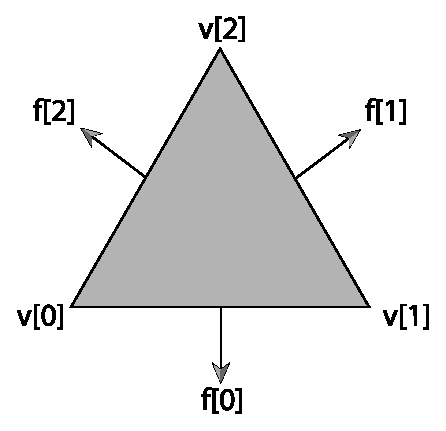
\includegraphics[width=0.35\linewidth]{chap03/Subdivvertfacepointers.eps}
    \caption{每个三角形面存有三个指向\protect\refvar{SDVertex}{}对象的
    指针{\ttfamily\protect\refvar[SDFace::v]{v}{}[i]}以及三个
    指向相邻面的指针{\ttfamily\protect\refvar[SDFace::f]{f}{}[i]}。
    相邻面索引使用的约定是第{\ttfamily i}边是
    从{\ttfamily\protect\refvar[SDFace::v]{v}{}[i]}到{\ttfamily\protect\refvar[SDFace::v]{v}{}[(i+1)\%3]}的边,
    且第{\ttfamily i}边的邻居在{\ttfamily\protect\refvar[SDFace::f]{f}{}[i]}中。}
    \label{fig:3.27}
\end{figure}

\begin{lstlisting}
`\refcode{LoopSubdiv Local Structures}{+=}\lastnext{LoopSubdivLocalStructures}`
struct `\initvar{SDFace}{}` {
    `\refcode{SDFace Constructor}{}`
    `\refcode{SDFace Methods}{}`
    `\refvar{SDVertex}{}` *`\initvar[SDFace::v]{v}{}`[3];
    `\refvar{SDFace}{}` *`\initvar[SDFace::f]{f}{}`[3];
    `\refvar{SDFace}{}` *`\initvar{children}{}`[4];
};
\end{lstlisting}

\refvar{SDFace}{}构造函数很简单——它简单地把这些不同的指针设置为{\ttfamily nullptr}——
所以这里不再展示。

为简化\refvar{SDFace}{}的数据结构导航,
我们提供宏使得决定特定索引前后的顶点和面索引更容易。
这些宏添加适合的偏移量并计算模三结果以负责循环。
\begin{lstlisting}
`\initcode{LoopSubdiv Macros}{=}`
#define `\initvar{NEXT}{}`(i) (((i) + 1) % 3)
#define `\initvar{PREV}{}`(i) (((i) + 2) % 3)
\end{lstlisting}

除了需要流形网格外,细分代码希望用户指定的控制网格
是\keyindex{相容次序}{consistently ordered}{}的——
网格中的每条\keyindex{有向边}{directed edge}{edge边}只能出现一次。
\subsection{细分}\label{sub:细分}